% ============================================================================
% Capítulo 7 — Projeto do banco de dados
% ============================================================================
\section{PROJETO DO BANCO DE DADOS}

\subsection{Modelo de dados}

O banco de dados foi modelado em SQL Server 2022 e é composto por quatorze
tabelas de negócio, além da tabela de controle de migrations. O modelo segue a
terceira forma normal: cada fato é armazenado uma única vez, e as relações são
expressas por chaves estrangeiras com integridade referencial explícita. A
Tabela~\ref{tab:entidades} descreve as entidades e seu papel no domínio.

\begin{table}[H]
  \centering
  \caption{Entidades do modelo de dados}
  \label{tab:entidades}
  \fontsize{9.5}{11.5}\selectfont
  \begin{tabular}{L{3.4cm}L{11.6cm}}
    \toprule
    \textbf{Entidade} & \textbf{Descrição} \\
    \midrule
    Cooperativa & Organização que agrega produtores e comercializa a produção \\
    Produtor & Agricultor associado, com comunidade de origem e situação de
      cadastro \\
    Produto & Item comercializável, com categoria, unidade e preço base \\
    LoteColheita & Quantidade colhida de um produto por um produtor, com código
      de rastreio \\
    Pedido & Compra realizada por um usuário comprador, com endereço de entrega \\
    ItemPedido & Produto e lote que compõem o pedido, com quantidade, preço e
      subtotal \\
    Rota & Programação de entrega com data, motorista e veículo \\
    Entrega & Unidade de entrega vinculada a um pedido e, opcionalmente, a uma
      rota \\
    Fatura & Documento de cobrança gerado a partir do pedido \\
    Motorista & Condutor habilitado a realizar rotas \\
    Veiculo & Veículo utilizado nas rotas, com placa e capacidade \\
    MovimentoEstoque & Entrada, saída ou ajuste de quantidade em um lote \\
    LogAcesso & Registro de auditoria de ações relevantes \\
    Usuario & Conta de acesso, com papel e estado \\
    \bottomrule
  \end{tabular}

  \vspace{2pt}
  {\fontsize{10}{12}\selectfont\itshape Fonte: elaborado pelo autor (2026)}
\end{table}

\subsection{Modelo entidade-relacionamento}

A Figura~\ref{fig:mer} apresenta o modelo entidade-relacionamento simplificado,
com as principais entidades e cardinalidades. As relações refletem as regras de
negócio: um produtor pertence a uma cooperativa; um lote referencia um produtor
e um produto; um pedido possui vários itens, e cada item pode referenciar um
lote; um pedido origina uma entrega e, quando faturado, uma fatura; e uma rota
agrupa várias entregas.

\begin{figure}[H]
  \centering
  \caption{Modelo entidade-relacionamento simplificado}
  \label{fig:mer}
  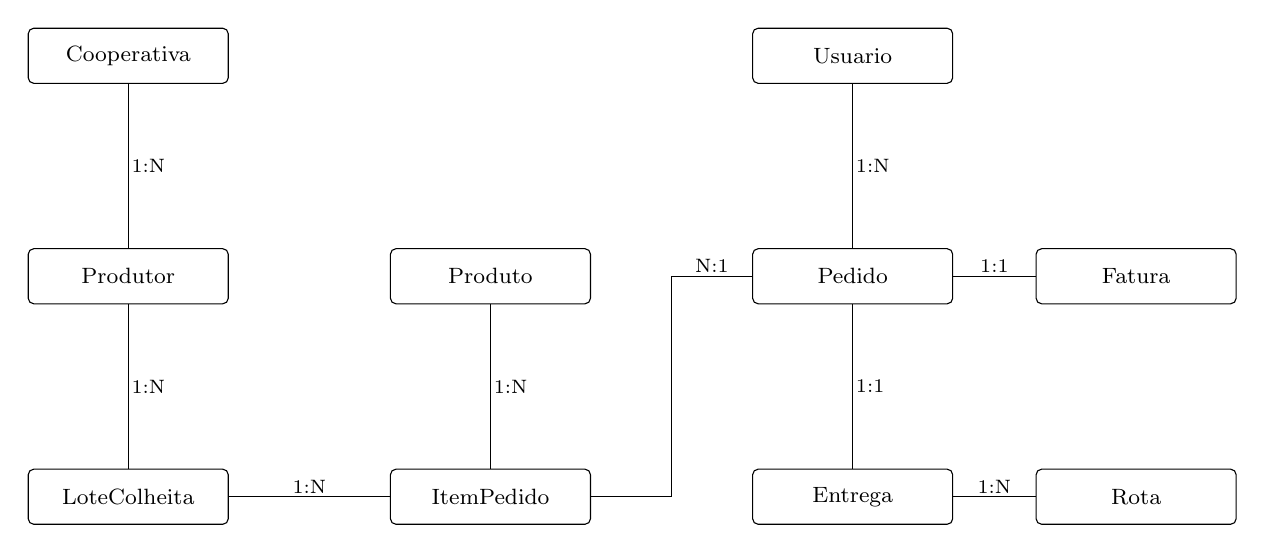
\begin{tikzpicture}[
    ent/.style={draw, rounded corners=2pt, align=center, font=\fontsize{8}{9}\selectfont,
      minimum height=7mm, text width=24mm, inner sep=2pt},
    linha/.style={thin},
    rot/.style={font=\fontsize{7.5}{8.5}\selectfont, fill=white, inner sep=1pt}
  ]
    \node[ent] (coop) at (0,9.0) {Cooperativa};
    \node[ent] (prod) at (0,6.2) {Produtor};
    \node[ent] (lote) at (0,3.4) {LoteColheita};

    \node[ent] (produto) at (4.6,6.2) {Produto};
    \node[ent] (item) at (4.6,3.4) {ItemPedido};

    \node[ent] (usuario) at (9.2,9.0) {Usuario};
    \node[ent] (pedido) at (9.2,6.2) {Pedido};
    \node[ent] (entrega) at (9.2,3.4) {Entrega};
    \node[ent] (fatura) at (12.8,6.2) {Fatura};
    \node[ent] (rota) at (12.8,3.4) {Rota};

    \draw[linha] (coop) -- node[rot, right] {1:N} (prod);
    \draw[linha] (prod) -- node[rot, right] {1:N} (lote);
    \draw[linha] (lote) -- node[rot, above] {1:N} (item);
    \draw[linha] (produto) -- node[rot, right] {1:N} (item);
    \draw[linha] (item.east) -- (6.9,3.4) -- (6.9,6.2) -- node[rot, above] {N:1} (pedido.west);
    \draw[linha] (usuario) -- node[rot, right] {1:N} (pedido);
    \draw[linha] (pedido) -- node[rot, right] {1:1} (entrega);
    \draw[linha] (pedido) -- node[rot, above] {1:1} (fatura);
    \draw[linha] (rota) -- node[rot, above] {1:N} (entrega);
  \end{tikzpicture}
  \fonte{elaborado pelo autor (2026)}
\end{figure}

\subsection{Dicionário de dados}

As tabelas a seguir detalham os principais atributos. Os campos de auditoria
(\texttt{CriadoEm} e \texttt{AtualizadoEm}) estão presentes em todas as tabelas e
foram omitidos do dicionário para evitar repetição.

\begin{table}[H]
  \centering
  \caption{Dicionário de dados --- Usuario}
  \label{tab:dic-usuario}
  \fontsize{9}{10.5}\selectfont
  \begin{tabular}{L{2.6cm}L{2.6cm}L{4.4cm}L{4.6cm}}
    \toprule
    \textbf{Campo} & \textbf{Tipo} & \textbf{Restrição} & \textbf{Descrição} \\
    \midrule
    Id & int & PK, identity & Identificador \\
    Nome & nvarchar(150) & obrigatório & Nome completo \\
    Email & nvarchar(200) & obrigatório, único & Login do usuário \\
    SenhaHash & nvarchar(255) & obrigatório & Hash PBKDF2 da senha \\
    Papel & nvarchar(20) & obrigatório & Admin, Produtor, Comprador ou Motorista \\
    Ativo & bit & obrigatório & Indica se a conta pode autenticar \\
    \bottomrule
  \end{tabular}

  \vspace{2pt}
  {\fontsize{9}{10.5}\selectfont\itshape Fonte: elaborado pelo autor (2026)}
\end{table}

\begin{table}[H]
  \centering
  \caption{Dicionário de dados --- Produtor e LoteColheita}
  \label{tab:dic-produtor}
  \fontsize{9}{10.5}\selectfont
  \begin{tabular}{L{2.6cm}L{2.6cm}L{4.4cm}L{4.6cm}}
    \toprule
    \textbf{Campo} & \textbf{Tipo} & \textbf{Restrição} & \textbf{Descrição} \\
    \midrule
    UsuarioId & int & FK $\rightarrow$ Usuario & Conta vinculada ao produtor \\
    CooperativaId & int & FK $\rightarrow$ Cooperativa & Cooperativa do associado \\
    NomePropriedade & nvarchar(150) & obrigatório & Nome da propriedade rural \\
    Documento & nvarchar(30) & obrigatório & CPF ou CNPJ \\
    Cidade / UF & nvarchar & obrigatório & Localização \\
    Comunidade & nvarchar(30) & obrigatório & Tradicional, Quilombola,
      Assentamento, Indígena ou Outro \\
    StatusCadastro & nvarchar(20) & obrigatório & Pendente ou Aprovado \\
    \midrule
    CodigoRastreio & uniqueidentifier & único & Código do lote \\
    ProdutorId & int & FK $\rightarrow$ Produtor & Origem do lote \\
    ProdutoId & int & FK $\rightarrow$ Produto & Produto colhido \\
    DataColheita & date & obrigatório & Data da colheita \\
    Quantidade & decimal(18,3) & $> 0$ & Quantidade colhida \\
    Status & nvarchar(20) & obrigatório & Disponivel, Esgotado ou Cancelado \\
    \bottomrule
  \end{tabular}

  \vspace{2pt}
  {\fontsize{9}{10.5}\selectfont\itshape Fonte: elaborado pelo autor (2026)}
\end{table}

\begin{table}[H]
  \centering
  \caption{Dicionário de dados --- Pedido, ItemPedido e Entrega}
  \label{tab:dic-pedido}
  \fontsize{9}{10.5}\selectfont
  \begin{tabular}{L{2.6cm}L{2.6cm}L{4.4cm}L{4.6cm}}
    \toprule
    \textbf{Campo} & \textbf{Tipo} & \textbf{Restrição} & \textbf{Descrição} \\
    \midrule
    CompradorId & int & FK $\rightarrow$ Usuario & Autor do pedido \\
    DataPedido & datetime2 & obrigatório & Data e hora do pedido \\
    Status & nvarchar(30) & obrigatório & Pendente, EmRota, Entregue ou Cancelado \\
    ValorTotal & decimal(18,2) & $\geq 0$ & Soma dos subtotais \\
    EnderecoEntrega & nvarchar(300) & obrigatório & Local de entrega \\
    \midrule
    PedidoId & int & FK $\rightarrow$ Pedido & Pedido do item \\
    ProdutoId & int & FK $\rightarrow$ Produto & Produto vendido \\
    LoteId & int & FK $\rightarrow$ LoteColheita & Lote de origem \\
    Quantidade & decimal(18,3) & $> 0$ & Quantidade do item \\
    PrecoUnitario & decimal(18,2) & $\geq 0$ & Preço praticado \\
    Subtotal & decimal(18,2) & $\geq 0$ & Quantidade $\times$ preço \\
    \midrule
    PedidoId & int & FK $\rightarrow$ Pedido & Pedido entregue \\
    RotaId & int & FK $\rightarrow$ Rota & Rota da entrega \\
    DataPrevista & date & obrigatório & Data prevista \\
    DataRealizada & datetime2 & nulo até a conclusão & Data efetiva \\
    Latitude / Longitude & float & nulo até a evidência & Coordenadas \\
    FotoUrl & nvarchar(500) & nulo até a evidência & Caminho da foto \\
    \bottomrule
  \end{tabular}

  \vspace{2pt}
  {\fontsize{9}{10.5}\selectfont\itshape Fonte: elaborado pelo autor (2026)}
\end{table}

\subsection{Procedimentos armazenados}

Três procedimentos concentram cálculos que precisam ser consistentes para
qualquer cliente. O \texttt{sp\_CalcularTotalPedido} recalcula subtotais e total
do pedido; o \texttt{sp\_ConsolidarEstoqueLote} consolida entradas, saídas,
ajustes e saldo de um lote; e o \texttt{sp\_RelatorioVendasProdutor} produz o
relatório de vendas por produtor em um intervalo de datas. A
Tabela~\ref{tab:procs} resume os parâmetros e o resultado de cada um.

\begin{table}[H]
  \centering
  \caption{Procedimentos armazenados}
  \label{tab:procs}
  \fontsize{9.5}{11.5}\selectfont
  \begin{tabular}{L{4.8cm}L{3.6cm}L{6.6cm}}
    \toprule
    \textbf{Procedimento} & \textbf{Parâmetros} & \textbf{Retorno} \\
    \midrule
    \texttt{sp\_CalcularTotalPedido} & \texttt{@PedidoId} & Atualiza subtotais
      e valor total \\
    \texttt{sp\_ConsolidarEstoqueLote} & \texttt{@LoteId} & Entradas, saídas,
      ajustes e saldo do lote \\
    \texttt{sp\_RelatorioVendasProdutor} & \texttt{@ProdutorId},
      \texttt{@DataInicio}, \texttt{@DataFim} & Itens vendidos e totais por
      pedido \\
    \bottomrule
  \end{tabular}

  \vspace{2pt}
  {\fontsize{10}{12}\selectfont\itshape Fonte: elaborado pelo autor (2026)}
\end{table}

O trecho a seguir reproduz o núcleo do procedimento de consolidação, que trata
cada tipo de movimento com sinal próprio para calcular o saldo.

\begin{lstlisting}[language=SQL]
SELECT lote.Id, lote.CodigoRastreio, lote.Quantidade,
       ISNULL(SUM(CASE WHEN m.Tipo = 'Entrada' THEN m.Quantidade END), 0) AS Entradas,
       ISNULL(SUM(CASE WHEN m.Tipo = 'Saida'   THEN m.Quantidade END), 0) AS Saidas,
       ISNULL(SUM(CASE m.Tipo WHEN 'Entrada' THEN m.Quantidade
                              WHEN 'Saida'   THEN -m.Quantidade
                              WHEN 'Ajuste'  THEN m.Quantidade
                              ELSE 0 END), 0) AS Saldo
  FROM dbo.LoteColheita AS lote
  LEFT JOIN dbo.MovimentoEstoque AS m ON m.LoteId = lote.Id
 WHERE lote.Id = @LoteId
 GROUP BY lote.Id, lote.CodigoRastreio, lote.Quantidade;
\end{lstlisting}

\subsection{Gatilhos}

Os gatilhos garantem que determinados efeitos ocorram independentemente do
cliente que altera os dados. O \texttt{trg\_Entrega\_LogStatus} registra em
\texttt{LogAcesso} toda mudança de status de entrega; o
\texttt{trg\_ItemPedido\_MovimentoEstoque} cria o movimento de saída quando um
item é inserido; e o \texttt{trg\_Produtor\_AuditaAprovacao} registra a mudança
de situação do cadastro. A Tabela~\ref{tab:triggers} sintetiza essas regras.

\begin{table}[H]
  \centering
  \caption{Gatilhos implementados}
  \label{tab:triggers}
  \fontsize{9.5}{11.5}\selectfont
  \begin{tabular}{L{5.3cm}L{2.6cm}L{7.1cm}}
    \toprule
    \textbf{Gatilho} & \textbf{Tabela} & \textbf{Efeito} \\
    \midrule
    \texttt{trg\_Entrega\_LogStatus} & Entrega & Registra status anterior e
      novo na auditoria \\
    \texttt{trg\_ItemPedido\_MovimentoEstoque} & ItemPedido & Cria movimento de
      saída do lote \\
    \texttt{trg\_Produtor\_AuditaAprovacao} & Produtor & Registra aprovação ou
      reprovação do cadastro \\
    \bottomrule
  \end{tabular}

  \vspace{2pt}
  {\fontsize{10}{12}\selectfont\itshape Fonte: elaborado pelo autor (2026)}
\end{table}

O trecho a seguir reproduz o gatilho que registra em auditoria as mudanças de
status de entrega.

\needspace{13\baselineskip}
\begin{lstlisting}[language=SQL]
CREATE OR ALTER TRIGGER dbo.trg_Entrega_LogStatus
ON dbo.Entrega AFTER UPDATE AS
BEGIN
    SET NOCOUNT ON;
    IF TRIGGER_NESTLEVEL() > 1 RETURN;

    INSERT INTO dbo.LogAcesso (UsuarioId, Acao, Entidade, EntidadeId, UserAgent, CriadoEm)
    SELECT NULL, CONCAT('StatusEntrega:', d.Status, '->', i.Status),
           'Entrega', CAST(i.Id AS NVARCHAR(60)), 'trigger', SYSUTCDATETIME()
      FROM inserted AS i
      INNER JOIN deleted AS d ON d.Id = i.Id
     WHERE i.Status <> d.Status;
END;
\end{lstlisting}

\subsection{Integridade, índices e script de criação}

A integridade é garantida em três níveis: tipos e restrições de verificação
(\emph{check constraints}) impedem valores inválidos, como quantidade negativa
ou preço inferior a zero; chaves estrangeiras impedem referências órfãs, com
políticas de exclusão coerentes (cascata para itens e fatura, preservação para
lotes e produtos); e índices em chaves estrangeiras e colunas de filtro aceleram
as consultas mais frequentes, como pedidos por comprador e entregas por
motorista.

O script \texttt{db/script-completo.sql} reúne a criação das tabelas, dos
procedimentos, dos gatilhos e da carga de demonstração, permitindo reconstruir o
banco em um ambiente limpo com um único comando. A validação foi executada em
contêiner SQL Server 2022: o script criou 15 tabelas (14 de negócio e a de
histórico de migrations), 3 procedimentos e 3 gatilhos, e as rotinas foram
exercitadas com dados reais -- o cálculo do pedido resultou em R\$ 425,00, a
consolidação do lote apresentou saldo de 70 unidades e o relatório de vendas
retornou os itens do período. As migrations do EF Core também foram aplicadas em
banco vazio, confirmando a equivalência entre o modelo de código e o script.
